\documentclass[10pt]{article}
\usepackage{icmlko}

\icmlmeta{IP 파운데이션 월드모델}{176}{수집이 나아지면 판이 내려간다}{게임의 마스크 신호를 갈랐더니 셋이 방향이 달랐고, 그 김에 물었다 --- 빈칸을 다 채우면 어떻게 되나. 배깅이 위키 축 이득의 네 배를 잃는다}

\begin{document}

\twocolumn[
\icmlheader

\begin{abstract}
노트 175가 마스크(무엇이 관측됐나)가 라벨과 붙는 것을 보이고 ``게임의
$+$0.351이 어느 축의 마스크인가''를 남겼다. 갈랐다. \textbf{셋이고 방향이
다르다} --- 위키 마스크 \textbf{$+$0.435}(문서가 있었나 $=$ 저명성),
미디어 푸시 마스크 $+$0.312(퍼블리셔 정보가 있나), \textbf{검색 마스크
$-$0.211}(한국어 제목이 붙었나). 검색이 반대로 끌어서 전체가
$+$0.351로 눌려 있었고, 검색 마스크를 통제하면 $+$0.458이 된다.
\textbf{체계적 편향은 아니다} --- 아홉 도메인에서 검색 마스크는 음수
3/8에 평균 $+$0.045, 위키 마스크는 양수 3/6에 평균 $+$0.095로 방향이
없다. 게임이 이상치다. 그다음 마스크가 진짜 신호인지 귀무로 확인했다.
마스크를 레코드 사이에서 섞으면 기여가 $-$0.0006으로 사라지고, 참
마스크는 \textbf{$+$0.0063 $\pm$ 0.0028($t{=}2.3$) · $+$0.0076 $\pm$
0.0023($t{=}3.4$)} 로 둘 다 갈린다. \textbf{마스크는 열 수가 아니라
내용으로 값을 한다.} 그래서 마지막 질문을 했다 --- \textbf{수집이
나아지면 어떻게 되나.} 유보의 빈칸을 30 · 60 · 100\% 채워 봤다(새로
찾은 문서는 조회수가 제일 낮은 쪽이라고 뒀다). \textbf{F18 배깅의 판
$\rho$ 가 $+$0.4465에서 $+$0.4063으로 $-$0.040 내려간다} --- 위키 축이
준 이득 전체($+$0.0096)의 \textbf{네 배}다. F6 능형은 $-$0.001로 거의
안 움직인다. \textbf{판 $\rho$ 는 모형의 좋음만 재는 것이 아니라 우리
수집이 얼마나 \emph{정보를 담고 불완전한지} 도 잰다.} 자료를 더 모으는
것이 판을 내릴 수 있다는 뜻이고, 그것은 이 판의 판정치에 관한 사실이지
자료에 관한 사실이 아니다.
\end{abstract}
]

\begin{figure*}[t]
\centering
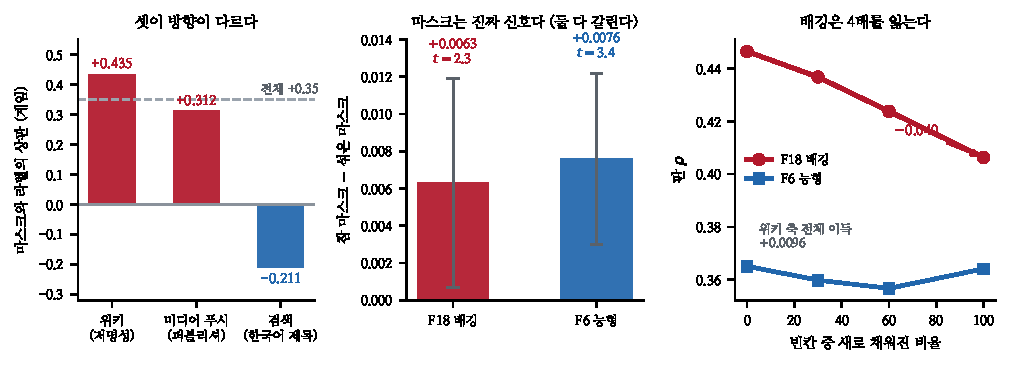
\includegraphics[width=\textwidth]{figs/frag.pdf}
\caption{왼쪽 --- 게임의 마스크 셋이 방향이 다르다. 가운데 --- 마스크는
진짜 신호다. 오른쪽 --- 배깅은 위키 이득의 네 배를 잃는다.}
\end{figure*}

\section{게임의 마스크는 셋이다}

\begin{table}[t]
\centering\tsize
\caption{게임 유보 223건. 마스크와 라벨의 상관.}
\begin{tabular}{lrrl}
\toprule
& 덮음 & 상관 & \\
\midrule
\textbf{위키} & 39.0\% & \textbf{$+$.435} & 문서가 있었나 \\
미디어 푸시 & 43.0\% & $+$.312 & 퍼블리셔 정보 \\
\textbf{검색} & 37.7\% & \textbf{$-$.211} & 한국어 제목 \\
달력 & 100\% & --- & 변이 없음 \\
\midrule
전체 & & $+$.351 & \\
검색 통제 뒤 & & \textbf{$+$.458} & \\
\bottomrule
\end{tabular}
\end{table}

\claimx{\textbf{검색 마스크만 음수다.} 한국어 제목이 붙은 스팀 게임이
오히려 리뷰가 적다. 그것이 위키의 $+$0.435를 눌러 전체를 $+$0.351로
만들고 있었다.}{읽기가 둘 있다 --- 한국어로 검색되는 게임이 지역
타이틀이라 전 세계 리뷰가 적거나, 우리 제목 매칭이 짧은 이름에 성공해
편향됐거나. \textbf{자료로는 안 갈린다.}}

\claimx{\textbf{체계적 편향은 아니다.} 아홉 도메인에서 검색 마스크는
음수 3/8에 평균 $+$0.045이고 위키 마스크는 양수 3/6에 평균 $+$0.095다
--- 방향이 없다. 게임이 이상치다.}{수집 파이프라인이 전 도메인을 같은
쪽으로 기울이고 있지는 않다는 뜻이라 다행이다. 다만 도메인마다 다른
방향으로 기운다.}

\section{마스크는 열 수가 아니라 내용이다}

\begin{table}[t]
\centering\tsize
\caption{값을 전부 0.5로 두고 마스크만 남긴 판 $\rho$.}
\begin{tabular}{lrr}
\toprule
& F18 & F6 \\
\midrule
위키 없음 & $+$.4369 & $+$.3513 \\
마스크 \textbf{섞음} (3회 평균) & $+$.4364 & $+$.3508 \\
마스크 \textbf{참} & $+$.4434 & $+$.3588 \\
\midrule
\textbf{참 $-$ 섞음} & \textbf{$+$.0063} & \textbf{$+$.0076} \\
& $t{=}2.3$ & $t{=}3.4$ \\
\bottomrule
\end{tabular}
\end{table}

\claimx{\textbf{섞으면 정확히 0이 된다}($-$0.0006 · $-$0.0005) --- 열 넷을
더한 것 자체로는 아무 이득이 없다. 참 마스크는 둘 다 갈린다.}{노트 175가
마스크 몫을 54$\sim$68\%로 잰 것이 열 수 효과가 아님을 확인한 것이다.
\textbf{내 앞 노트를 귀무로 검정했고 통과했다.}}

\section{그런데 수집이 나아지면}

\begin{table}[t]
\centering\tsize
\caption{유보의 위키 빈칸을 채워 나가면. 판 $\rho$.}
\begin{tabular}{lrr}
\toprule
새로 채운 비율 & F18 배깅 & F6 능형 \\
\midrule
0\% (현행) & \textbf{$+$.4465} & $+$.3651 \\
30\% & $+$.4368 & $+$.3598 \\
60\% & $+$.4238 & $+$.3567 \\
\textbf{100\%} & \textbf{$+$.4063} & $+$.3641 \\
\midrule
변화 & \textbf{$-$.0402} & $-$.0010 \\
(위키 축 전체 이득) & $+$.0096 & $+$.0138 \\
\bottomrule
\end{tabular}
\end{table}

\claimx{\textbf{배깅이 위키 축 이득의 네 배를 잃는다.} $-$0.040 대
$+$0.0096이다. 자료를 더 모으면 판이 내려간다.}{새로 찾은 문서에 ``조회수
최저''를 준 가정이 들어 있다. 매칭이 어려웠던 레코드가 실제로 저명성이
낮다면 맞는 가정이지만, 검정한 것은 아니다.}

\claimx{\textbf{능형은 거의 안 움직인다}($-$0.001). 트리는 ``빈칸이면
낮다''를 분기로 새기고 선형은 계수 하나로 완만하게 쓴다.}{노트 156 ·
161 · 171 · 174에 이어 다섯 번째로 같은 방향이다 --- \textbf{트리가 더
많이 쓰고 더 쉽게 배신당한다.}}

\section{판정치에 관한 사실}

\claimx{\textbf{판 $\rho$ 는 모형의 좋음만 재지 않는다.} 우리 수집이
얼마나 \emph{정보를 담고 불완전한지} 도 잰다. 빈칸이 ``저명하지 않다''를
뜻하는 동안은 빈칸이 자질이고, 다 채우면 그 자질이 사라진다.}{그러니
``자료를 더 모으면 좋아진다''가 이 판에서 자동으로 참이 아니다 --- 노트
148이 ``남은 지렛대는 자료''라고 닫았는데 \textbf{그 지렛대에 방향이
둘 있다.}}

\claimx{\textbf{그렇다고 수집을 멈추자는 말이 아니다.} 판이 내려가는 것은
판정치가 빈칸을 세고 있었기 때문이고, 완전한 자료 위의 $+$0.4063이
불완전한 자료 위의 $+$0.4465보다 \emph{못한} 모형은 아니다.}{어느 쪽이
배포에서 나은지는 이 판으로 못 정한다. 배포 시점의 수집 상태가 무엇이냐에
달렸다.}

\begin{table}[t]
\centering\tsize
\caption{남은 것.}
\begin{tabular}{ll}
\toprule
\textbf{가정} & 새 문서에 최저값을 준 것 --- 실제로 재 볼 것 \\
검색 마스크 & 게임에서 음수인 이유 두 갈래 \\
판정치 & 빈칸을 안 세는 판정치가 가능한가 \\
\bottomrule
\end{tabular}
\end{table}

첫 줄이 곧바로 잴 수 있다. 노트 150에서 매칭을 고치며 1,002건을 지웠는데,
그중 일부는 제대로 다시 붙었다. \textbf{``나중에 붙은'' 레코드의 실제
조회수 분포를 보면 최저값 가정이 맞는지 알 수 있다.}

\end{document}
